\subsection{Language Concepts}\label{sec:langconcepts}

\newcommand{\fcontrolflow}{\f{ControlFlow}}
\newcommand{\fmodularity}{\f{Modularity}}
\newcommand{\fdatatypes}{\f{DataTypes}}
\newcommand{\fevents}{\f{EventSupport}}
\newcommand{\freadsensor}{\f{ReadSensor}}
\newcommand{\fcontrolflowparadigm}{\f{ControlFlowParadigm}}
\newcommand{\factions}{\f{Actions}}
\newcommand{\fexceptions}{\f{ExceptionHandling}}
\newcommand{\ffileaccess}{\f{FileAccess}}
\newcommand{\ffunctionlib}{\f{FunctionLibrary}}
\newcommand{\fmultithread}{\f{Multithreading}}

We found a range of different concepts offered by the languages for specifying missions. We consider a concept a distinct element of the abstract syntax of the language. We focus on concepts that are recognizable via the notation (concrete syntax), since many of our environments are not open-source, preventing a look at the exact implementation of the language's abstract syntaxes. End-users observe these concepts via the language's notation and utilize them via the respective projectional editor, except for the textual additional languages provided by some environments. As shown in \figref{fig:langconcepts}, we classified the concepts we found into the features: \fcontrolflow, \fmodularity, \fdatatypes, \fevents, \freadsensor, \fcontrolflowparadigm, \factions, \fexceptions, \ffileaccess, \ffunctionlib, and \fmultithread, as detailed below.

%Language concepts is a sub-feature of languages that %is treated separately because it 
%highlights the concepts that determine the expressiveness of the language while specifying missions. Sub-features of the language concepts include: control flow, modularity of the language, variable data types supported, event support ability, the types of sensor data that can be read, control flow paradigm, actions the robots can perform, exception handling, file access feature, function libraries, and multithreading support.

%The expressive power of the environments is determined by the language concepts that are salient to the end-user. As shown in \figref{fig:langconcepts}, we categorized these concepts into control flow, modularity concepts, variable data types, event support, read sensor, control flow paradigms, actions, exception handling, file access, function  library, and multi-threading.  

\begin{figure}[t]
     \centering
    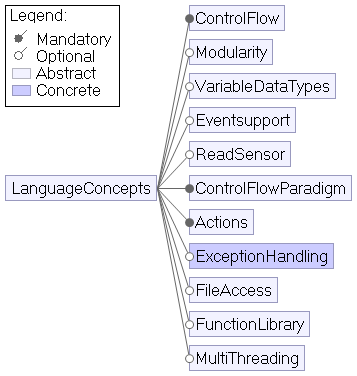
\includegraphics[width=.6\columnwidth]{LanguageConcepts.png}
      \caption{Language Concepts%\tb{change VariableDataTypes to DataTypes}
      }
      \label{fig:langconcepts}
			\vspace{-.4cm}
   \end{figure}

\parhead{\fcontrolflow.} The languages offer several kinds of control-flow statements, such as, conditionals (\texttt{if-do}, \texttt{if}, \texttt{if-else}, and \texttt{switch}), loops (e.g., \texttt{do-while}, \texttt{while}, \texttt{forever}, \texttt{repeat while}, \texttt{repeat count} in \lego, figure \ref{fig:controlFlow} and \texttt{repeat until} in figure \ref{fig:robotcgraphical}), and loop interrupts (\texttt{loop interrupt} in \lego, \texttt{stop all} in \tello, \texttt{wait (time/event), break, and until})%\tb{I need concrete examples here, since the writeup is not systematic enough}.
\begin{figure}[t]
     \centering
    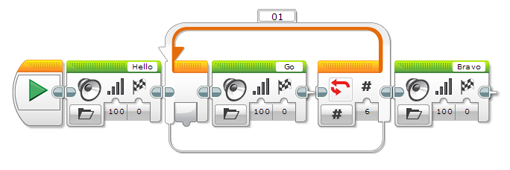
\includegraphics[width=1\columnwidth]{legoLoop.png}
      \caption{Program control flow example in \lego. \emph{(robot say "Hello" once, then "Go" six times, then "Bravo" once)}%\tb{change VariableDataTypes to DataTypes}
      }
      \label{fig:controlFlow}
			\vspace{-.4cm}
   \end{figure}


Multi-threading controls are also found in \trik (\texttt{fork}, \texttt{join}, \texttt{kill thread}), in  \lego for running tasks simultaneously (\texttt{sequence plug exit}) and in \robotmesh, for example in blockly,  \texttt{start block} creates s thread, \texttt{sleep for x seconds} forces thread to yield. %\tb{also need an example here}.

\parhead{Modularity.} Despite our environments being user-oriented, the majority offers modularization concepts (e.g., functions) to structure larger missions. We found functions, which are graphically represented using dedicated blocks, in the environments called functions, procedures or modules; each havina a

 Modularity focuses at mission sub-components that are used to accomplish specific tasks.
Examples include \metabot, \ardublockly, \openroberta, \choregraphe, \sphero, \robotmesh, \metabot, \makeblock, \ozoblockly, and \turtlebot; they create mission modules using functions and function calls. \choregraphe implements robot behaviors as boxes, which are connected in a flow chart to form a mission. \lego imports blocks from external environments that are compatible with \lego. \trik implements subprograms, functions, and module with symbolic icon of what these components do; in this way they become mission modules. \picaxe implements procedures of particular concepts, which then can be invoked and used.  \missionlab has predefined states used to build a state machine for a given mission. 

%https://www.tivipe.com/2016/08/30/merging-modules/#more-461

\parhead{Variable data types.} While \flyaq, \missionlab, \tivipe, and \trik do not have exclusive variable data types, the rest of the environments has primitive types and compound data types. The primitive types include integer, decimal, character, float, number, and boolean, while compound types include strings/text, arrays, table, and lists. Other types include sound in \ozoblockly, logic (true, false) in \lego, degrees in \tello, and color in \sphero. In \aseba, state is a variable type;  for instance temperature is a variable that can take values like off, low, medium, high, and light is a variable that can take values like on and off. 

\parhead{Function libraries} - Function libraries offer functions and operation on data, including complex algorithms used to process data. Most environments provide function libraries for mathematics, logic and string operation; however \missionlab, \flyaq, \aseba, \codelab, and \tello do not offer such libraries. 

%\parheadit{Examples}
Top provide some examples, the logic functions include comparison like and/or, not, true/false, null, and test. The math sub-feature includes mathematics function, calculating parameters, trigonometric function, constant, number property, change by x, round, list evaluation, remainder of, constrain, random (integer, fraction), squareroot, return constant(sqrt, pi,...), sum of list, array operations, and range. Text operations include create, append, build string, length, find occurrence in a list, get sublist, is empty, get letter, get substring, join, and letter 1 of.  %Math box and data edit box in \choregraphe.     

\parhead{Control flow paradigm} - This determines how missions are executed, which can take the form of imperative execution, reactive paradigm or goal based. In imperative execution, the mission runs in the order of sequence of the tasks specified, which is the common paradigm of most environments in this study. However, \aseba Visual Programming features a reactive paradigm in which events, which act as triggers are matched with corresponding actions, which categorize it as a reactive. In some of the imperative environments like \picaxe, reactive aspects are also realized as robot, which responds to sensor data during mission execution. We did not come across an environment, which follows a goal-based control-flow paradigm.

 
\parhead{Actions} - These are activities robots execute to achieve a given task. Some are reactions to events, while others are activities that are imperatively specified in the mission. We classified robot actions as action type, actuation action, communication action, and movement actions. Robot actions  can be instantaneous actions e.g. take photo~\cite{FLYAQ}, pause, resume~\cite{PICAXE}, or continuous action e.g. follow line~\cite{LEGO,Sphero}, or timed executions where duration of execution is measured with start/stop time or events, like record a video~\cite{FLYAQ}. The actuation actions refer to device/actuator wise actions like grasp an object, motor movements, audio play. Communication actions include interacting with humans and non-human agents.  Communication with humans can be of the form of text, video, or audio. While non-human agents can  be categorized as tuple space, publish-subscribe or message passing. Tuple space is a shared space where shared data items are kept for access to entities entitled to access them, publish-subscribe where publishers avail messages regardless of receivers while subscribers receive messages they have subscribed to.
Movement actions manage mobility of robots. Languages offer concepts that specify how a robot moves from one location to another. Such  concepts are either absolute ``map coordinates", or relative like direction, distance, or travel time.\\
%\parheadit{Actuation examples identified} - 

Actuation examples include get button code, play tones, sound, stop motors, clear encoder, angular servo, turn on LED, detection with videocamera, line detector, video streaming enabling, beep note, buzzer, display, status light, object observation, taping, face status (smile, frown), among others. %lift, backpack, speak, think, change color, hide number, change volume, screen print, screen draw(line/object), start timer, set robot state, say hello, stand-up, wave with hand, move, DoPhoto, monitor street (road task), Intercept Object, LeaveRoom, Localize position, LookForObject, MarkNearestObject, MarkNearestDoor, MoveAhead, MoveAway, MOveForward, MoveToward, PickUp, SurveryRoom, Talk, Terminate, TrackTarget, Wait, Wander, follow line, gripper(open, close, stop), set mode(active, rest, sit). \patrizio{not sure we need all this}\\ 
 
%\parheadit{Action type examples}
Action type examples include the ``random eyes duration ms" block that is used in \openroberta to turn NAO's eye LEDS to change eye color for specified duration in milliseconds. Instead in NXT the ``get value ms timer" block is used as a sensor to read current time for another block, while the ``reset timer" block is used to reset the internal timer to zero. Similar time constructs also exist in other environment, like the wait time and elapsed time blocks in \ardublockly, the set roll time in seconds as a variable, time elapsed, get current time, set timeout, set time interval in \sphero, the set timer(seconds), timer, wait(seconds), wait until (event) in \vex among others. \\

%\parheadit{Communication examples} 
Communication example include infrared messages exchanged among robots in  \edison, \lego, and \openroberta, and Bluetooth messages exchange between bricks in Lego Ev3. In \missionlab, when in GOTO state, robots share information about target goal position and map of the environment among each other directly or through broadcasts. \sphero, \vex, \makeblock, and \tello broadcast message between robots. \flyaq supports synchronization and communication messaging among drones at run time.  \trik supports sending message to other robots. For what concerns human and central system to robot communications, examples are hand-clap and touch in \aseba, and \enchanting, send text, send number, send command, receive character, send character, send, and receive message in \tello, speak short phrase in \codelab, say text in \trik, \tivipe from the robot to the environment. In \choregraphe robot can share text with humans. In \arcbotics, humans interact with robot through beep, status led colors, infrared remote code and \picaxe communicates through infrared messages. Eleven of the 29 environments do not offer any communication language constructs. \\

%\parheadit{Movement examples} 
Few of the environments support absolute movement actions, such as e.g. goto (coordinates) in \flyaq, \missionlab, \makeblock, moveto (coordinates), movefast (coordinates, duration) in \tivipe, roll(angle, speed, time), spin(angle, time in seconds) in \sphero, drive (distance) in \codelab. For relative movements we mention go/move/drive/turn/fly (forward/backward/left/right/room) as seen in most of the environments like \metabot, \trik, and \lego.

\parhead{Event support} - Event support considers language abilities to handle events like creating event handlers, the types of events that can be recognized, and mechanisms of synchronizing events to subsequent actions. The common language constructs for event support identified include when (event), when (event) do, wait for (event), wait until (event), wait (event), on (event), capture(event), move until (event), broadcast and wait 9event) in \vex, AtGoal, AtEndOfHall, in \missionlab, and delay (event). The events are sensory data that trigger the next robot action. However environments like \arcbotics, \tivipe, \minibloq, \turtlebot, and \robotc do not have event support language constructs.\\

\parhead{Read Sensor} - From the environment the robot captures data through sensor readings, which inform robots next action. Much as most environments offered language support to capture respective sensor data, \turtlebot and \missionlab do not offer language concepts to manipulate sensors while \choregraphe supports vision recognition using vision reco box and sound recognition using speech reco box. \ozoblockly uses proximity sensor concept to detect objects without details of the sensor.\\

%\parheadit{Example} 
Common sensors captured in the environments include gyro for measuring rotations, light/light intensity, sound/clap detector, touch, temperature/thermometer, ultrasonic for measuring distance, timer, compass, accelerometer, gesture detector, and face recognizer. Other sensors are sonar, infrared ranger, GPS module, finger print scanner, motor rotation counter, energy meter, line detector, angle reader, line tracker, potentiometer, velocity, power(wats), current (amps), magnetometer, and force resister. The number of sensors on the robot and nature of the missions the robot is designed for determine the language constructs for the sensors.  \\

\parhead{Exception Handling} - Only three environments, namely \openroberta, \choregraphe, and \codelab offer support for exception handling in their text notation but none in the graphical notation. %\tb{probably just very few, right?} 

%\parheadit{Examples} 
More specifically, \openroberta exploits the Python exception handler, and \choregraphe exploits the try catch block for all errors in C++ software development kit (SDK) and the try catch block for face detection error in python SDK. \codelab offer support for exception handling for the following errors: actionerror, animations not loaded, can not place objects on this, connection aborted, connection check failed, connection error, no devices found, not pickupable, and robot busy.\\

\parhead{File Access} - It is a block found in \lego, used for reading and writing data from and to memory, close or delete a file. Such file can record for instance ambient light measurements taken at given time intervals, which are stored in memory and can be displayed on the LCD display screen ~\cite{LEGO}. \trik allows writing to robot file system, \choregraphe supports open, close and save operations to file while \missionlab offers read, write, close and delete language construct for file operations. \picaxe also supports read and write operations. The rest of the environments do not offer any language support for file access operations.

\parhead{Multithreading} - This concept when supported by a language enables users to do several activities without waiting for one activity to end. This improves speed of execution especially when it involves user. In \robotmesh,  using blockly editor,  \textit{start} block creates s thread, \textit{sleep} for x seconds forces thread to \textit{yield}, \textit{start autonomous} creates a thread that runs in autonomous mode of the robot, \textit{start driver} creates a thread that runs in driver mode. In python, sys.run\_in\_thread(f), sys.thread\_id(), sys.sleep(t). In C++, thread (void (*callback)(void)), get\_id(), join(), interrupt(), yield(), sleep\_for(unit32\_t time\_ms), lock(), try\_lock(), unlock(). \trik offers fork, join, kill thread, send message to thread functions to execute multithreading. \lego offers Sequence Plug Exit block for creating parallel tasks, though the simultaneous tasks need to be manually verified to avoid resource conflicts. \makecode and \robotc use \textit{run in parallel} block to support multithreading of mission tasks. \tivipe uses \textit{splitSCIS} to split and run three modules  in parallel. \missionlab supports Cthread, which is a lightweight process threads package from Georgia Tech which operates under Linux, SunOS operating systems. While \picaxe supports multi-tasking with operations like; restart, resume, and suspend.












  %\begin{figure}[h]
% \subsection{How the environments differ}
% \noindent
% General language features ~\cite{Clark}; notation is the concrete syntax of a language expressed either as textual syntax or visual syntax. Abstract syntax describes the vocabulary of the concept and how they are combined, while semantics describes what the language represents and means. Mapping feature describes how the language translates to other languages, its semantic equivalence, abstraction level with respect to similar languages and also internal mapping of the abstract syntax to concrete syntax as part of the language architecture. While extensibility of the language states how the language handles adding new concepts to boost its expressiveness. By considering features as end-user visible characteristics of the system, the environments can be compared based on; notation, extensibility, semantics and some aspects of mapping.
% Feature matrix\\
% $\bullet$ Notation matrix\\
% $\bullet$ coupling and reuse of mission artifacts in different contexts\\
% $\bullet$ control flow at run time; imperative (sequence and branch, in concurrent threads, reactive to events or declarative)\\
% editing features (syntax, semantic 

% What made the environments different\\
% $\bullet$ \parhead{Based on underlying technology} blockly based, scratch based, or generic \\
% $\bullet$ \parhead{Connection of blocks} flow chart based or nonflow chart (no links between blocks)\\
% $\bullet$ \parhead{Closeness of mapping} icon based or regular graphical blocks\\
% $\bullet$ \parhead{User domains} students focused (learning), electro-mechanical domain with features of electronics components like motors, programming domains demonstratting features of programming languages,\\ 
% $\bullet$ \parhead{Semantics} are the languages interpreted or compiled. The common generated code languages including; Java Script, Java, C/C++, Python.\\
% $\bullet$ \parhead{Control flow Vs Data flow based}. Control flow based languages graphical languages organize functional blocks into directed graph using arrows. A current block executes command and passes control to the next block based on the output generated. While in data flow based languages, program blocks are data variables that receive data from sensor system, whose value determines the next course of action ~\cite{Mordvinov2017}.
% ======================
% To be crosschecked~\cite{crosscheck}

% \begin{itemize}
% %In robotics, who specifies the mission requirements? (user domain expert, robotic engineer)
%     \item Task features; behavioral/functional model
%     \item Environmental features
%     \item Performance metrics; governing rules that constrain the behavior of the task
%     \item Robot capabilities; physical parts(actuators) that exhibit the behavior of the task
%     \item Mission goal; user goal, purpose of the mission
%     \item Single robot or team of robots mission, if multi-robots, the task distribution/delegation strategy (automatic or explicitly specified).This also includes interactive missions where humans work with robots.
%     \item In quantitative specifications, execution times for respective tasks should be specified otherwise sequence of specification for qualitative specifications.This can be an input to motion planning unit.
%      \item Text; type or select from drop-down list
%     \item Visual/graphical; point at locations to visit in a map, drag and drop domain primitive icons to define sequence of events.
%     \item Audio interaction with robot
%     \item task specification tree where nodes are declarative specification of tasks to perform\cite{Doherty2013}. Can missions be decomposed to tasks and subtasks to form a task forest or bigger tree? Weintrop et al \cite{Weintrop2018} reports use of trees to hierarchically program tasks. Robot routine is broken  into  a series of steps, with each step having sub steps, resulting into hierarchical program as implemented in universal robots' polyscope interface.
% \end{itemize} 
% \claudio{Can you try to put here for each RQ the concepts that aims at answering that RQ. For example, 
% RQ1: Debugging, Simulator.}
% \claudio{If you collected something that is not mapped to an RQ you have two options:
% 1 - you drop it. Because the information is not useful
% 2 - you add a new RQ.}